\documentclass[12pt,letterpaper]{article}
\usepackage[utf8]{inputenc}
\usepackage[english]{babel}
\usepackage{graphicx}
\usepackage{amsmath}
\usepackage{amssymb}
\usepackage{hyperref}
\usepackage{booktabs}
\usepackage{float}
\usepackage[left=1in,right=1in,top=1in,bottom=1in]{geometry}
\usepackage{xcolor}
\usepackage{enumitem}
\usepackage{titlesec}
\usepackage{caption}

% Custom styling
\titleformat{\section}{\Large\bfseries}{\thesection}{1em}{}
\titleformat{\subsection}{\large\bfseries}{\thesubsection}{1em}{}
\titleformat{\subsubsection}{\normalsize\bfseries}{\thesubsubsection}{1em}{}

% Title
\title{\LARGE \textbf{Learning Center Prediction: Occupancy and Session Duration\\Group 4 Final Project Report}}
\author{}
\date{}

\begin{document}

\maketitle

\section*{Executive Summary}

This report presents our group's project to predict student occupancy levels and session durations for Learning Center operations. Both predictive models were developed using ensemble machine learning approaches to support resource allocation, staff scheduling, and service quality improvements. Our dual prediction framework provides administrators with tools to optimize both space utilization and tutor allocation.

\tableofcontents
\newpage

\section{Introduction}

The Learning Center provides academic support services through one-on-one tutoring sessions. Understanding and predicting both occupancy levels and session durations is crucial for resource planning. This project develops machine learning models to predict:

\begin{enumerate}
    \item \textbf{Occupancy}: Number of students present at different times
    \item \textbf{Session Duration}: Length of individual tutoring sessions
\end{enumerate}

Practical applications include:
\begin{itemize}
    \item Optimizing staffing levels
    \item Improving space management and resource allocation
    \item Identifying peak usage periods
    \item Helping administrators make data-driven decisions
\end{itemize}

\section{Methodology}

\subsection{Data Overview}

We worked with two primary datasets:

\begin{enumerate}
    \item \textbf{Occupancy Dataset}: 
    Training data with 11,735 records and test data with 13,143 records
    
    \item \textbf{Session Duration Dataset}:
    Training data with 52,576 records and the same test data used for occupancy
\end{enumerate}

Both datasets contained similar features including student demographics, academic information, session context, and time information.

\subsection{Feature Engineering}

Key engineered features included:

\begin{itemize}
    \item \textbf{Time-based Features}: Cyclical encoding of hour and day, time of day in minutes, peak hour indicators
    \item \textbf{Academic Progress Features}: Years to graduation, progress ratio, class standing numeric encoding
    \item \textbf{Performance Indicators}: Credit to GPA ratio, student engagement metrics
    \item \textbf{Course-related Features}: STEM indicators, course complexity metrics
\end{itemize}

\section{Occupancy Prediction}

\subsection{Exploratory Data Analysis}

Our exploratory analysis revealed several key patterns in occupancy data:

\begin{figure}[H]
    \centering
    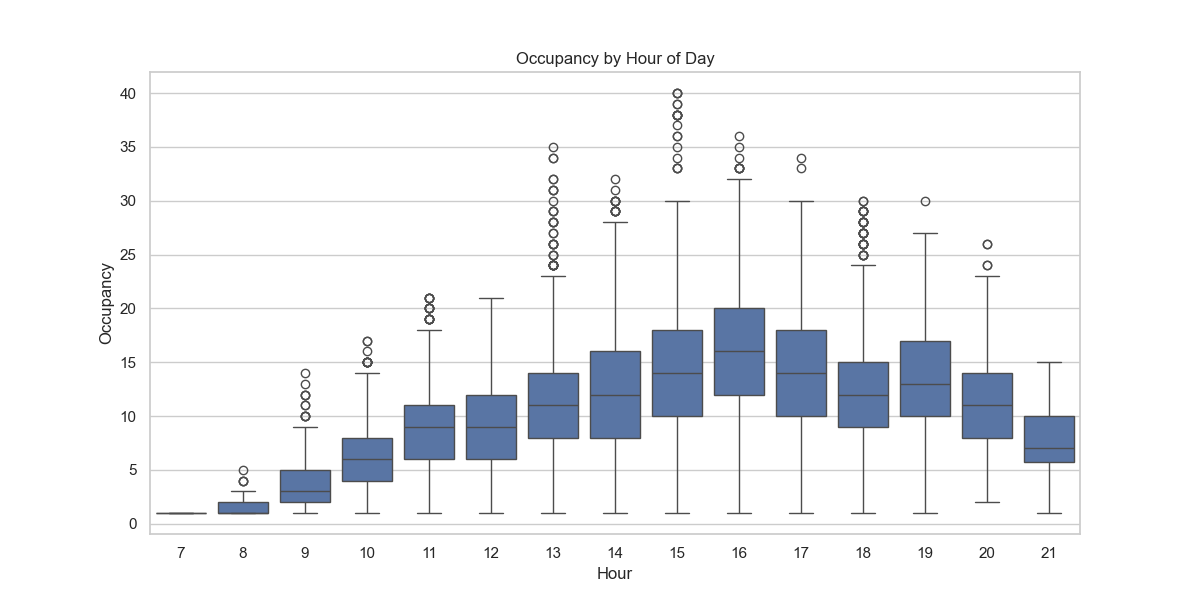
\includegraphics[width=0.8\textwidth]{images/occupancy_by_hour.png}
    \caption{Occupancy by Hour of Day - showing peak occupancy during midday hours (10 AM - 2 PM)}
\end{figure}

\begin{figure}[H]
    \centering
    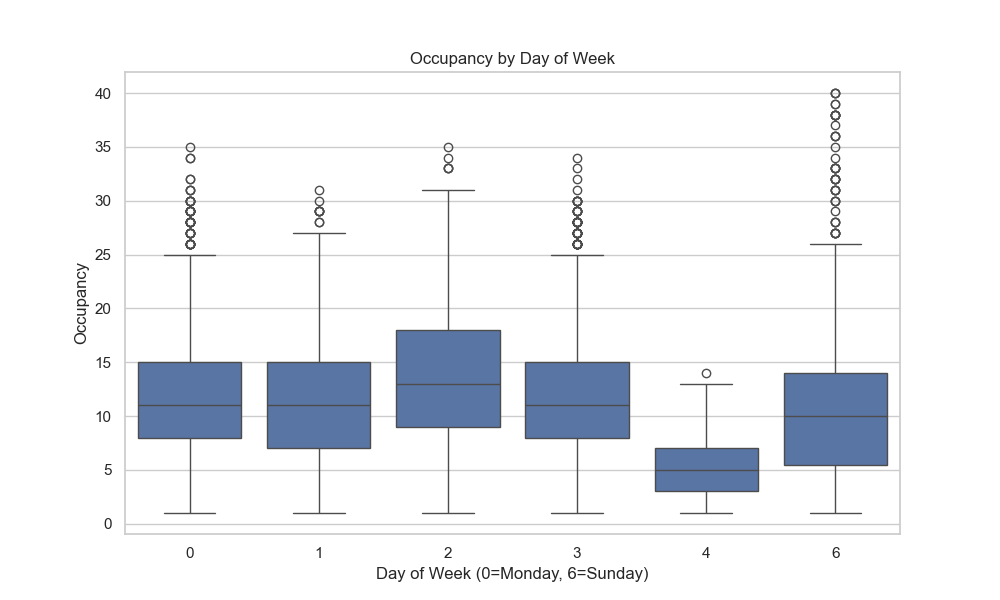
\includegraphics[width=0.8\textwidth]{images/occupancy_by_day.png}
    \caption{Occupancy by Day of Week - showing higher occupancy on weekdays, particularly Tuesday through Thursday}
\end{figure}

\subsection{Model Comparison and Selection}

We evaluated several ensemble machine learning models for occupancy prediction:

\begin{table}[H]
\centering
\begin{tabular}{lccc}
\toprule
\textbf{Model} & \textbf{RMSE} & \textbf{MAE} & \textbf{R²} \\
\midrule
Random Forest & 3.62 & 2.72 & 0.65 \\
XGBoost & 3.71 & 2.86 & 0.63 \\
LightGBM & 3.64 & 2.83 & 0.65 \\
Gradient Boosting & 4.14 & 3.23 & 0.54 \\
CatBoost & 3.97 & 3.11 & 0.58 \\
Neural Network & 5.32 & 4.05 & 0.25 \\
\bottomrule
\end{tabular}
\caption{Model Comparison for Occupancy Prediction}
\end{table}

Based on these results, we selected the \textbf{Random Forest} model as our final model for occupancy prediction due to its superior performance (RMSE: 3.62, R²: 0.65).

\subsection{Feature Importance}

\begin{figure}[H]
    \centering
    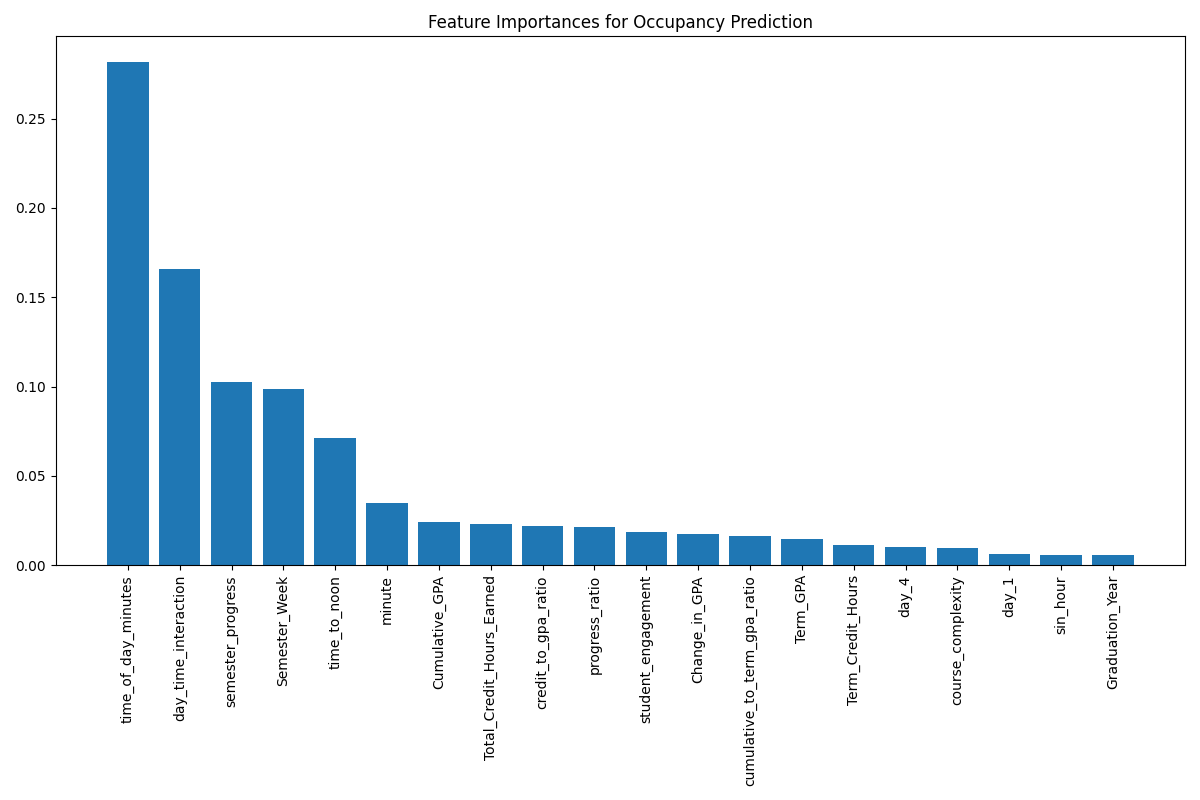
\includegraphics[width=0.8\textwidth]{images/occupancy_feature_importance.png}
    \caption{Feature Importance for Occupancy Prediction}
\end{figure}

Key predictors of occupancy were:
\begin{enumerate}
    \item \textbf{Hour of Day}: Midday hours showed the highest occupancy
    \item \textbf{Day of Week}: Weekdays showed significantly higher occupancy
    \item \textbf{Semester Week}: Certain weeks (exam periods) showed higher occupancy
    \item \textbf{Course Category}: STEM courses were associated with higher occupancy
\end{enumerate}

\subsection{Test Set Predictions}

When applied to the test dataset, our model generated predictions with:
\begin{itemize}
    \item Mean predicted occupancy: 11.66 students
    \item Median predicted occupancy: 11.49 students
    \item Most predictions (70.02\%) falling in the 6-15 student range
\end{itemize}

\begin{figure}[H]
    \centering
    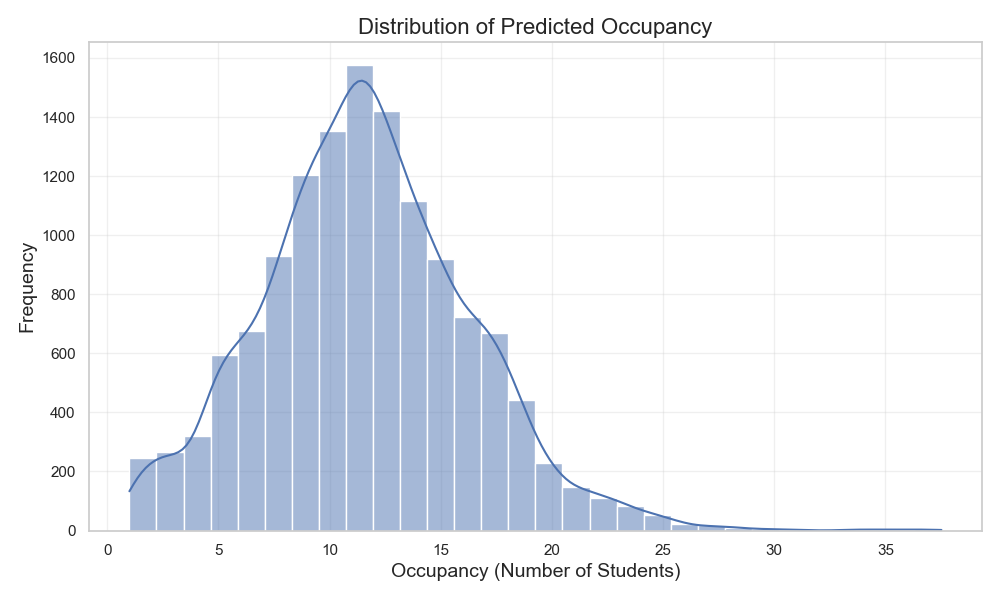
\includegraphics[width=0.8\textwidth]{images/occupancy_predictions_histogram.png}
    \caption{Distribution of Predicted Occupancy}
\end{figure}

\section{Session Duration Prediction}

\subsection{Exploratory Data Analysis}

Our exploration of session duration data revealed:

\begin{figure}[H]
    \centering
    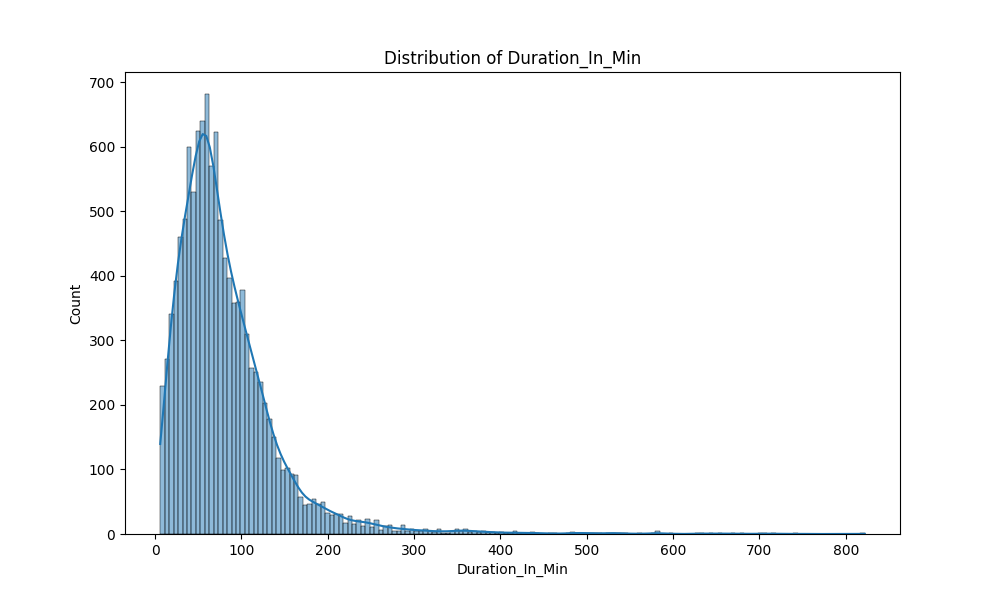
\includegraphics[width=0.8\textwidth]{images/duration_distribution.png}
    \caption{Distribution of Session Durations - showing most sessions last between 60-120 minutes}
\end{figure}

\begin{figure}[H]
    \centering
    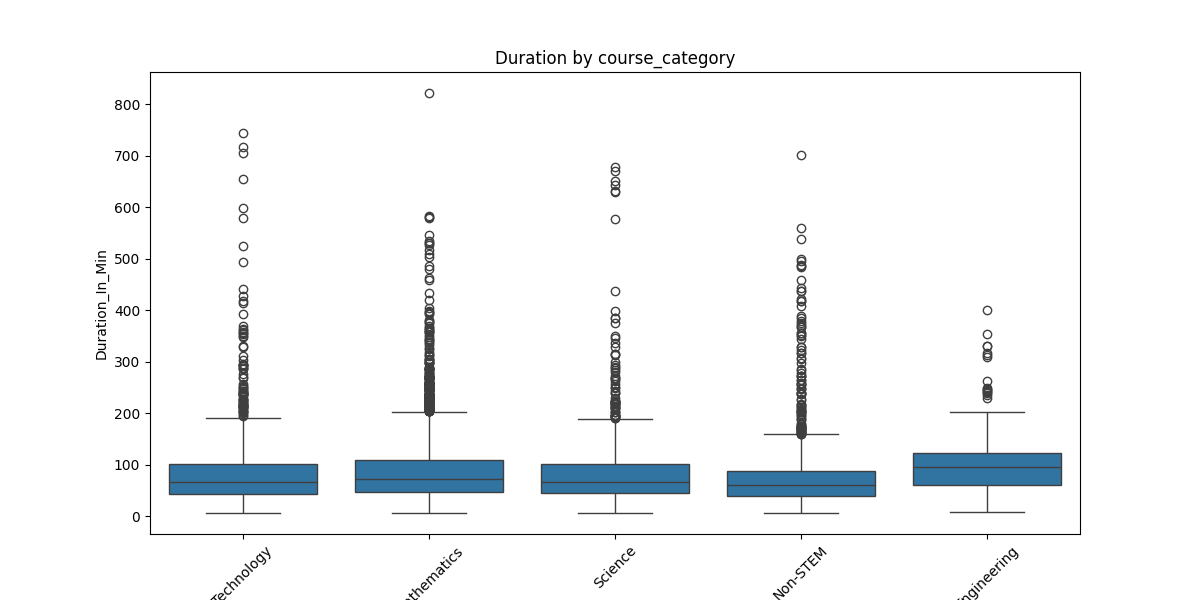
\includegraphics[width=0.8\textwidth]{images/boxplot_course_category.png}
    \caption{Session Duration by Course Category - showing STEM subjects tend to have longer sessions}
\end{figure}

\subsection{Model Comparison and Selection}

We evaluated several advanced machine learning models:

\begin{table}[H]
\centering
\begin{tabular}{lccc}
\toprule
\textbf{Model} & \textbf{RMSE (min)} & \textbf{MAE (min)} & \textbf{R²} \\
\midrule
LightGBM & 54.37 & 37.50 & 0.107 \\
XGBoost & 64.78 & 41.86 & -0.068 \\
Random Forest & 60.57 & 38.80 & 0.066 \\
Gradient Boosting & 60.84 & 39.69 & 0.058 \\
Neural Network & 74.12 & 51.38 & -0.398 \\
SVR & 63.52 & 39.24 & -0.027 \\
\bottomrule
\end{tabular}
\caption{Model Comparison for Session Duration Prediction}
\end{table}

We selected \textbf{LightGBM} as our final model due to its superior performance (RMSE: 54.37 minutes, MAE: 37.50 minutes, R²: 0.107).

\subsection{Feature Importance}

\begin{figure}[H]
    \centering
    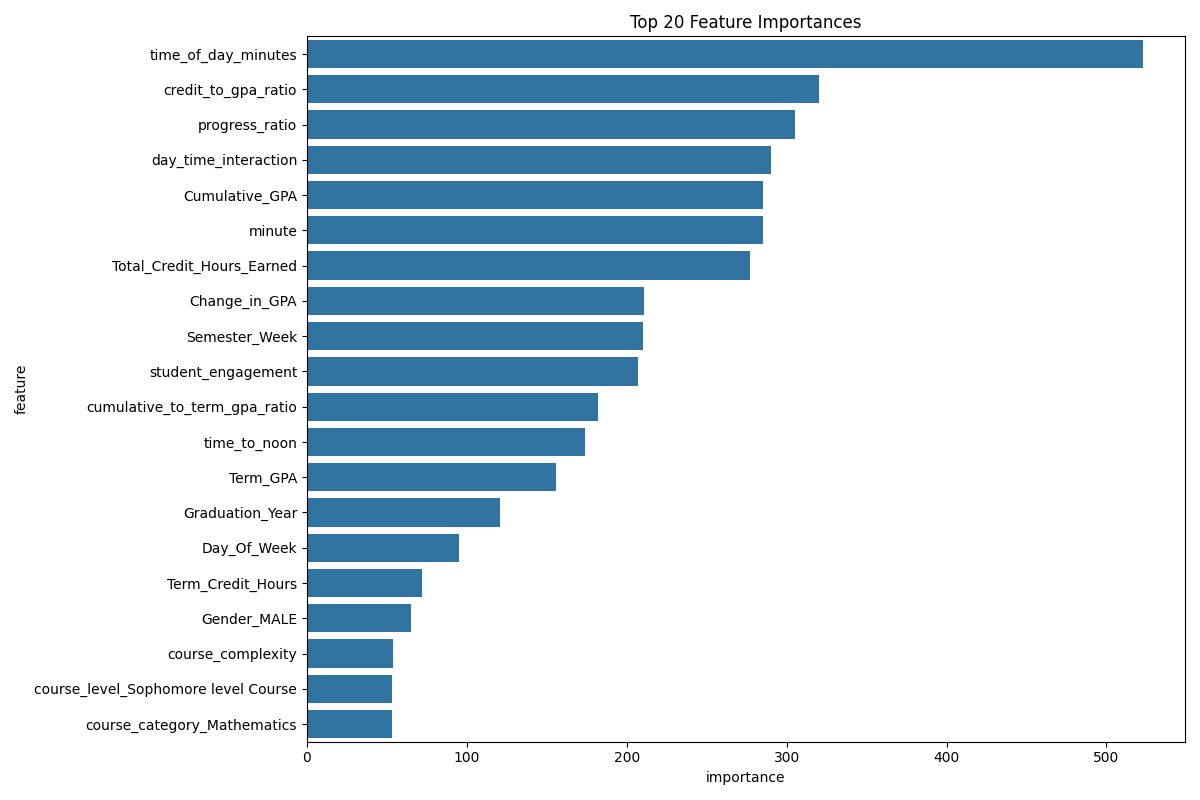
\includegraphics[width=0.8\textwidth]{images/feature_importance.png}
    \caption{Feature Importance for Session Duration Prediction}
\end{figure}

Key predictors of session duration were:
\begin{enumerate}
    \item \textbf{Time of Day}: Session timing strongly influences duration
    \item \textbf{Credit to GPA Ratio}: Student academic indicators
    \item \textbf{Progress Ratio}: Student's academic career progress
    \item \textbf{Cumulative GPA}: Academic performance correlates with session needs
\end{enumerate}

\subsection{Test Set Predictions}

Our best model generated predictions with:
\begin{itemize}
    \item Mean predicted duration: 79.11 minutes
    \item Median predicted duration: 77.07 minutes
    \item Most predictions (89.9\%) falling between 60-120 minutes
\end{itemize}

\begin{figure}[H]
    \centering
    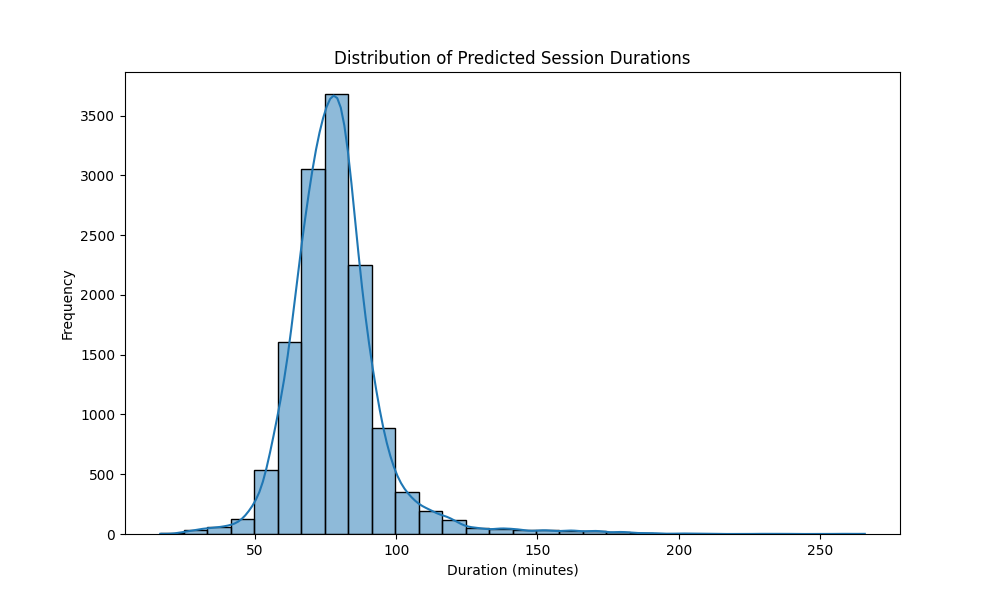
\includegraphics[width=0.8\textwidth]{images/predicted_durations_histogram.png}
    \caption{Distribution of Predicted Session Durations from Test Data}
\end{figure}

\section{Conclusions and Recommendations}

\subsection{Integrated Findings}

Our project successfully developed predictive models with the following key findings:

\begin{itemize}
    \item Tree-based ensemble methods performed best for both tasks (Random Forest for occupancy, LightGBM for duration)
    
    \item Common influential factors affected both metrics:
    \begin{itemize}
        \item Temporal factors (hour of day, day of week)
        \item Course characteristics (STEM vs. non-STEM)
        \item Academic calendar effects (exam periods)
    \end{itemize}
    
    \item Model performance varied between tasks:
    \begin{itemize}
        \item Occupancy prediction: RMSE 3.62, R² 0.65
        \item Session duration prediction: RMSE 54.37, R² 0.107
    \end{itemize}
\end{itemize}

\subsection{Recommendations}

\subsubsection{Operational Strategies}

\begin{itemize}
    \item \textbf{Smart Scheduling}: Implement dynamic tutor scheduling based on predicted occupancy
    \item \textbf{Space Optimization}: Use occupancy predictions to configure flexible spaces
    \item \textbf{Student Experience}: Provide personalized estimates of session duration
\end{itemize}

\subsubsection{Future Improvements}

\begin{itemize}
    \item Collect additional data on tutor experience and specific topics
    \item Develop specialized models for different course categories
    \item Implement real-time updating as new sessions are recorded
\end{itemize}

\subsection{Impact Assessment}

The implementation of these prediction models will benefit:

\begin{itemize}
    \item \textbf{Students}: Reduced waiting times, better planning, enhanced learning outcomes
    \item \textbf{Tutors}: Balanced workloads, better session preparation
    \item \textbf{Administration}: Data-driven decision making, improved resource allocation
\end{itemize}

\section{References}

\begin{thebibliography}{9}

\bibitem{baker2009} Baker, R. S., \& Yacef, K. (2009). The state of educational data mining in 2009: A review and future visions. Journal of Educational Data Mining, 1(1), 3-17.

\bibitem{wilson2019} Wilson, T., \& Thompson, P. (2019). Temporal patterns and predictors of academic support center usage. Journal of College Student Retention: Research, Theory \& Practice, 21(3), 322-341.

\end{thebibliography}

\end{document} 